\documentclass[12pt, a4paper]{report}

%====================== PACKAGES ======================
\usepackage[french]{babel}

\frenchbsetup{StandardLists=true}
\usepackage{enumitem}
\usepackage{pifont}

\usepackage[utf8x]{inputenc}
%\usepackage[latin1]{inputenc}

%pour gérer les positionnement d'images
\usepackage{float}
\usepackage{amsmath}
\DeclareMathOperator{\dt}{dt}
\usepackage{graphicx}
%\usepackage{tabularx}
\usepackage[colorinlistoftodos]{todonotes}
\usepackage{url}

%pour les informations sur un document compilé en PDF et les liens externes / internes
\usepackage[pdfborder=0]{hyperref}
\hypersetup{
	colorlinks = true
	}

%pour la mise en page des tableaux
\usepackage{array}
\usepackage{tabularx}
\usepackage{multirow}
\usepackage{multicol}
\setlength{\columnsep}{50pt}

%pour utiliser \floatbarrier
%\usepackage{placeins}
%\usepackage{floatrow}

%espacement entre les lignes
\usepackage{setspace}

%modifier la mise en page de l'abstract
\usepackage{abstract}

%police et mise en page (marges) du document
\usepackage[T1]{fontenc}
\usepackage[top=2cm, bottom=2cm, left=2cm, right=2cm]{geometry}

%Pour les galerie d'images
\usepackage{subfig}

\usepackage{pdfpages}

\usepackage{tikz}
\usetikzlibrary{trees}
\usetikzlibrary{decorations.pathmorphing}
\usetikzlibrary{decorations.markings}
\usetikzlibrary{decorations.pathreplacing,calligraphy}
%\usetikzlibrary{decorations}
\usetikzlibrary{angles, quotes}
\usepackage{verbatim}

\usepackage{appendix}

\usepackage{comment}

\usepackage{xcolor}

%\PreviewEnvironment{tikzpicture}
%\setlength\PreviewBorder{0pt}%

%====================== INFORMATION ET REGLES ======================

%rajouter les numérotation pour les \paragraphe et \subparagraphe
\setcounter{secnumdepth}{4}
\setcounter{tocdepth}{4}

\hypersetup{							% Information sur le document
pdfauthor = {Stephan Runigo},			% Auteurs
pdftitle = {électromagnétisme et relativité},			% Titre du document
pdfsubject = {électromagnétisme et relativité},		% Sujet
pdfkeywords = {relativité électromagnétisme},	% Mots-clefs
pdfstartview={FitH}}	% ajuste la page à la largeur de l'écran
%pdfcreator = {MikTeX},% Logiciel qui a crée le document
%pdfproducer = {} % Société avec produit le logiciel

%======================== DEFINITION COMMANDES ========================
%\newcommand{\si}[1]{\textsf{\textit {#1}}}
%\newcommand{\fsb}[1]{\textsf{\textbf {\footnotesize #1}}}
\newcommand{\ve}[1]{\overrightarrow{#1}}
\newcommand{\vt}[1]{\overrightarrow{\text{#1}}}
\newcommand{\tx}[1]{\text{#1}}
\newcommand{\bi}[1]{\textbf{\textit {#1}}}
\newcommand{\mc}[1]{$\mathcal{#1}$}
\newcommand{\wti}[1]{\widetilde{#1}}
\newcommand{\wtt}[1]{\widetilde{\text #1}}
%======================== DEBUT DU DOCUMENT ========================
%
\begin{document}
%
%régler l'espacement entre les lignes
\newcommand{\HRule}{\rule{\linewidth}{0.5mm}}
%
% Titre, résumé, ... %
%
%
\begin{titlepage}
%
~\\[1cm]

\begin{center}
%\includegraphics[scale=0.5]{./presentation/chambreABulle}
\end{center}

\textsc{\Large }\\[0.5cm]

% Title \\[0.4cm]
\HRule

\begin{center}
{\huge \bfseries Relativité restreinte et\\
électromagnétisme\\[0.4cm] }
\end{center}

\HRule \\[1.5cm]

\begin{center}
%\includegraphics[scale=0.3]{./presentation/ptoleme}
\end{center}

% Author and supervisor
\begin{minipage}{0.4\textwidth}
\begin{flushleft} \large
%\emph{Auteur:}\\
%Stephan \textsc{Runigo}
\end{flushleft}
\end{minipage}
\begin{minipage}{0.4\textwidth}
\begin{flushright} \large
\emph{Latex-iation:}\\
Stephan \textsc{Runigo}
\end{flushright}
\end{minipage}

\vfill
\begin{minipage}{0.4\textwidth}
\begin{flushleft} \large
Exercices de l'ENS extraits de https://www.phys.ens.fr/
\end{flushleft}
\end{minipage}
\begin{minipage}{0.4\textwidth}
\begin{flushright} \large
\end{flushright}
\end{minipage}

\vfill

% Bottom of the page
{\large \today}

\end{titlepage}

\newpage
\begin{center}
\Large
Résumé
\normalsize
\end{center}
\vspace{3cm}
\begin{itemize}[leftmargin=1cm, label=\ding{32}, itemsep=21pt]
\item {\bf Objet : } Mécanique Quantique.
\item {\bf Contenu : } Notes de cours.
\item {\bf Niveau requis : } Maitrise de sciences physiques.
\end{itemize}

\vspace{3cm} \large

Notes de cours rédigées en 1966 par Serge Haroche
\vspace{3cm}

http://enseignement.phys.ens.fr/spip.php?article110
\vspace{3cm}


%

%
% Table des matières
\tableofcontents
\thispagestyle{empty}
\setcounter{page}{0}
%
%espacement entre les lignes des tableaux
\renewcommand{\arraystretch}{1.5}
%
%====================== INCLUSION DES CHAPITRES ======================
%
~
\thispagestyle{empty}
%recommencer la numérotation des pages à "1"
\setcounter{page}{0}
\newpage
%
\newcounter{numero}

%% Sébastien Leurent , Marc Lilley & Sylvain Nascimbène 14 février 2012

\section{Relativité restreinte}
\subsection{Électromagnétisme et relativité galiléenne}

On considère une charge ponctuelle q dans un référentiel galiléen $\mathcal{R}$ où règnent un champ
électrique {\bf E} et un champ magnétique {\bf B} . On appelle {\bf u} sa vitesse dans ce référentiel.
On considère un second référentiel galiléen $\mathcal{R}$' en translation uniforme à la vitesse {\bf v} par rapport
au référentiel $\mathcal{R}$ . On note {\bf u'} la vitesse de la charge ponctuelle q dans le référentiel $\mathcal{R}$'. On appelle
{\bf E'} et {\bf B'} les champs électrique et magnétique dans ce référentiel.
\begin{enumerate}
  \item En tenant compte de l'invariance de la charge et du principe de relativité, exprimer les
forces de Lorentz {\bf F} et {\bf F'} agissant sur la charge q dans chacun des référentiels.
  \item Expliquer pourquoi la force exercée sur un système d'étude est invariante dans une transformation galiléenne. Déduire l'expression des champs {\bf E'} et {\bf B'} en fonction des champs {\bf E}
et {\bf B}.
\setcounter{numero}{\theenumi}\end{enumerate}
On considère l'expérience d'électrostatique présentée sur la figure 1. Une charge q est au repos
dans le référentiel du laboratoire. Cette charge est soumise à l'influence d'un fil infini portant
une densité de charge linéique $\lambda$.

\begin{center}
\vspace{0.3cm}
\begin{tikzpicture}
\draw[thick] (-4,0)--(4,0);
\draw[dashed] (-1,0)--(-1,2);
\draw (-1,2) node {$\bullet$} node [right] {$q$};
\draw (-1,1) node [left] {$r$};
\draw (2,0) node [above] {$\lambda$};
\end{tikzpicture}

\vspace{0.3cm}
Fig. 1: Charge q en interaction avec un fil chargé
\end{center}
\begin{enumerate}
\setcounter{enumi}{\thenumero} 
  \item Calculer les champs électrique et magnétique créés par le fil (à partir des équations de
Maxwell) dans le référentiel du laboratoire puis dans un référentiel en translation uniforme
à la vitesse v dans une direction parallèle au fil.
  \item Calculer l'expression de la force de Lorentz dans ces deux réferentiels et conclure.
\end{enumerate}

\subsection{Expérience de Michelson-Morley (1887)}

L'expérience de Michelson-Morley avait pour but de mettre en évidence la présence d'un hypothétique
éther dans lequel la Terre se déplace, et qui définit le référentiel d'inertie dans lequel la
lumière se propage à la vitesse c . Le résultat négatif de cette expérience est une des expériences
fondamentales qui ont mené à la relativité restreinte.
Le principe de l'expérience est de réaliser un interféromètre dit de Michelson (voir Fig. 2), qui
permet de comparer les temps d'aller-retour dans deux bras perpendiculaires de même longueur
L , lorsque ceux-ci sont en mouvement par rapport à l'éther. La longueur déployée des bras est de
L = 22 m . La source de lumière utilisée était une lampe à vapeur de Sodium de longueur d'onde
$\lambda$ = 589 nm . La Terre se déplace à v = 30 km.s −1 autour du Soleil.

\begin{center}
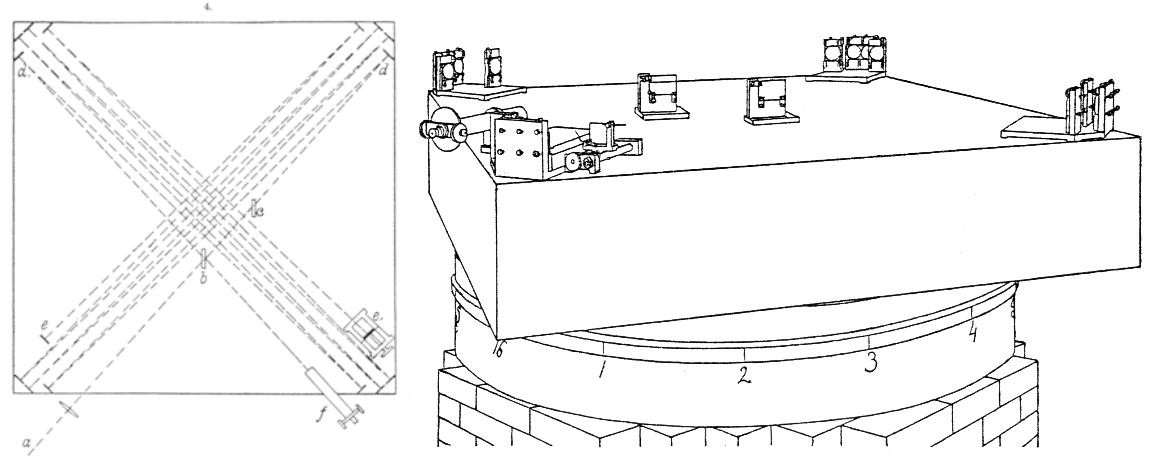
\includegraphics[scale=0.5]{./presentation/cropped-Michelson-morley-header}
%https://araz.community.uaf.edu/

Fig. 2: Principe et dispositif de l'expérience historique de Michelson-Morley.

{\it a : source lumineuse, b : lame semi-transparente, c : lame compensatrice, d : miroirs fixes, e : miroir réglable, f : occulaire}
\end{center}
\begin{enumerate}
  \item Effectuer un calcul de physique Galiléenne pour déterminer le temps d'aller retour d'un
flash lumineux le long de chacun des deux bras. On supposera que le mouvement de la
Terre coïncide avec la direction de l'un des bras.
  \item En déduire, dans la limite v ≪ c , le déphasage qui devrait être observé en sortie de l'interféromètre lorsqu'on éclaire l'interféromètre en lumière monochromatique. Comment observer
expérimentalement ce déphasage ?
  \item Le résultat de l'expérience historique a donné une absence de déphasage à mieux qu'un
centième de frange. Si l'éther existait, quelle serait sa vitesse maximale par rapport à la
Terre ? Commenter.
\end{enumerate}
\subsection{Désintégration de muons cosmiques}
Les muons sont des particules hargées ayant des propriétés très semblables aux éle trons excepté qu'ils sont plus massifs et instables. On les trouve en abondance dans les rayons cosmiques.
Leur durée de vie moyenne au repos a été mesurée et vaut : $\tau$ 0 = 2, 197 × 10 −6 s .
Un détecteur de muons est placé tout d'abord au sommet du Mont Washington (1910 m), puis
au pied de ette montagne, sensiblement au niveau de la mer. Dans sa première position, le
détecteur enregistre 563 +
− 10 muons par heure, dans sa seconde position, 408 +
− 9 .
\begin{enumerate}
  \item En faisant l'hypothèse que la vitesse des muons est proche de c , calculez leur durée de vie
moyenne $\tau$ telle qu'elle est mesurée par un expérimentateur terrestre.
En réalité, au cours de cette expérience, on a pu sélectionner des muons de vitesse v = 0, 992c .
  \item Montrez que l'expérimentateur peut retrouver cette valeur de $\tau$ à partir de la connaissance
de $\tau$ 0 .
\end{enumerate}
\subsection{Temps propre et temps impropre}
Une fusée quitte la Terre avec une vitesse $\beta$ ≡ v/c = 3/5 . Quand une horloge placée sur la
fusée indique qu'une heure s'est écoulée, la fusée envoie un signal lumineux à la Terre.
\begin{enumerate}
  \item Pour les horloges terrestres, quand le signal lumineux a-t-il été envoyé ?
  \item Pour les horloges terrestres, combien de temps après le départ de la fusée le signal a-t-il
atteint la Terre ?
  \item Pour les horloges de la fusée, combien de temps après le départ de la fusée le signal a-t-il
atteint la Terre ?
\end{enumerate}
\subsection{L'effet Doppler}
On considère une source ponctuelle S émettant des flashs lumineux sphériques à une fréquence
qui se propagent à la vitesse de la lumière c . Comme il est indiqué sur la Fig. 3, la source est
animée d'une vitesse v par rapport au référentiel du laboratoire, qui fait un angle $\theta$ avec l'axe
de visée (toujours dans le référentiel du laboratoire).
$\nu$ S '
S
v
q
r
O
Fig. 3 : Source S se déplaçant à la vitesse v par rapport à un observateur O fixe dans le référentiel
du laboratoire.
Un observateur immobile dans ce référentiel est placé au point O. On repère par le vecteur
r la position de la source qui a émis le signal présent en O. On suppose l'observateur éloigné,
c'est-à-dire r ≫ c/$\nu$ ' .
\subsubsection{Effet Doppler classique ( v ≪ c )}
\begin{enumerate}
  \item Dans le référentiel du laboratoire, exprimer la durée ∆t O séparant la réception de 2 flashs
pour l'observateur en fonction de ∆t S , période d'émission du signal dans le référentiel de
l'observateur.
  \item Interpréter graphiquement l'effet Doppler classique en représentant les crêtes correspondant
à 4 périodes successives sur un dessin. Y-a-t-il un effet Doppler classique transverse (pour
$\theta$ = $\pi$/2 ) ?
\setcounter{numero}{\theenumi}\end{enumerate}
\subsubsection{Effet Doppler relativiste}
\begin{enumerate}
  \setcounter{enumi}{\thenumero}
  \item Définir ensuite un référentiel dans lequel l'intervalle de temps séparant 2 flashs est un temps
propre et en déduire la fréquence $\nu$ O mesurée par l'observateur en fonction de v , $\theta$ et de la
fréquence $\nu$ S ' de la source.
\end{enumerate} 
\subsection{Diverses mesures de longueurs}
On considère une fusée voyageant à la vitesse v entre 2 planètes A et B séparées d'une distance L .
\begin{enumerate}
  \item Calculez l'intervalle de temps mesuré par une horloge de la fusée entre les 2 franchissements
de planètes.
  \item Déduisez en la longueur L ' mesurée par le pilote de la fusée entre les 2 planètes.
\setcounter{numero}{\theenumi}\end{enumerate}
On considère un appareil comportant une source d'éclairs E placée à égale distance de 2 miroirs
situés en A et B , eux-mêmes séparés d'une distance L (mesurée au repos). Comme il est indiqué
sur la figure 4, l'ensemble se déplace à une vitesse v par rapport au laboratoire.

La source émet un éclair au temps t = t ' = 0 juste quand elle passe devant le point E ' du
laboratoire. L'éclair atteint les points A et B , est réfléchi vers le laboratoire et laisse 2 marques
en A ' et B ' .
\begin{enumerate}
  \setcounter{enumi}{\thenumero}
  \item Trouvez les temps indiqués par des horloges situées en A , B , A ' et B ' quand l'éclair y arrive.
  \item Les événements : l'éclair est en A ' et l'éclair est en B ' sont-ils simultanés ?
\end{enumerate} 
Fig. 4 : Dispositif émettant un éclair en E et le réfléchissant en A et B .

%%TD n°2
\chapter{Voyage interstellaire}
Ce TD, qui regroupe un certain nombre d’applications de la transformation de Lorentz, a
pour but d’étudier quelques aspects du voyage à des vitesses proches de celle de la lumière. La
première partie permet de mettre en évidence le fameux paradoxe des jumeaux tel qu’il a été
formulé par le physicien Paul Langevin (1911). La deuxième partie propose un point de vue qui
permet de faire disparaître le paradoxe. Enfin, la dernière partie présente un modèle de voyage
plus réaliste que celui proposé précédemment.
\section{Paradoxe des Jumeaux} %1 
Deux jumeaux naissent sur Terre, l’un est appelé le sédentaire et noté S et l’autre est appelé
le voyageur et noté V. Dès leur naissance, les deux jumeaux sont séparés : pendant que S reste
sur la Terre, V monte dans une fusée piloté par le pilote P' et part pour une étoile E située à
une distance L $=$ 40 années-lumière de la Terre et effectue son voyage à la vitesse constante \bi{v}
(par rapport à la Terre) telle que $\gamma = 22$. On note \mc{R} le référentiel inertiel lié à la Terre dans
lequel S est au repos, et \mc{R'} le référentiel inertiel lié au pilote P'. Le point de départ est l’origine
O (x $=$ 0 et t $=$ 0) et le mouvement s’effectue selon l’axe O$x$ du référentiel \mc{R}. On notera T la
durée du voyage de la Terre à l’étoile dans le référentiel \mc{R}.
\begin{enumerate}
  \item Paramétrer les lignes d’univers de S, V et E dans chacun des deux référentiels \mc{R} et \mc{R'} .
Représenter les diagrammes d’espace-temps dans \mc{R} et \mc{R'} .
  \item Calculer la durée T du voyage vue par S puis la durée T' du voyage pour V.
\setcounter{numero}{\theenumi}\end{enumerate}
Les jumeaux S et V, connaissant un brin de relativité, savent que les temps de parcours T et
T' sont différents. Chacun des deux veut savoir quel est l’âge de l’autre lorsque le voyage aller
est terminé. L’âge de V pour S est déterminé ainsi : S demande à un observateur S$_2$ , lié à \mc{R} et
fixe sur l’étoile, de lire l’horloge de V à son arrivée sur l’étoile. De même, pour connaître l’âge
de S pour V, V demande à un observateur V$_2$ , lié à \mc{R'} et coïncidant avec S quand V arrive sur
l’étoile, de lire l’horloge de S.
\begin{enumerate}
  \setcounter{enumi}{\thenumero}
  \item Quels sont les âges de V pour S et de S pour V déduits de la procédure ci-dessus ? Quel
est le jumeau le plus jeune à l’arrivée de V sur l’étoile ? Pourquoi l’âge de S pour V mesuré
ainsi n’est pas égal à T ?
\setcounter{numero}{\theenumi}\end{enumerate} 
On s’intéresse maintenant au trajet retour : on suppose qu’à peine arrivé sur l’étoile, V saute
sur une seconde fusée pilotée par P'' , et qui se dirige à la vitesse $−$\bi{v} vers la Terre. On note \mc{R''}
le référentiel inertiel lié à P'' .
\begin{enumerate}
  \setcounter{enumi}{\thenumero}
  \item Quel est la durée du trajet retour pour S et pour V ? En déduire les temps d’aller-retour
T$_{AR}$[S] et T$_{AR}$[V] pour S et V.
  \item Voici le raisonnement de Langevin : « {\it le temps d’aller-retour} T$_{AR}$[S] {\it pour} S {\it est un temps
propre, il doit donc être égal à} $T_{AR}[V]/\gamma$. De même, le temps d’aller-retour T$_{AR}$[V] pour
V est un temps propre, il doit donc être égal à $T_{AR}[S]/\gamma$. {\it Ces deux phrases sont contradictoires si} $\gamma \neq 1$ ». Où est l’erreur dans le raisonnement de Monsieur Langevin ? Quelle
phrase est la bonne ?

{\footnotesize (Paul Langevin avait parfaitement compris la relativité restreinte et n’a jamais proposé le paradoxe des jumeaux
comme une preuve de l’inconsistance de la relativité restreinte. Au contraire, le « paradoxe » qui porte son
nom a en fait été porté devant ses contemporains par Langevin pour leur montrer que la notion de simultanéité
pouvait induire en erreur.)}
  \item Calculer, pour S, P' , P'' et V, la durée du voyage aller et celle du voyage retour. Proposer
deux méthodes pour le calcul du temps aller dans \mc{R''} et du temps retour dans \mc{R'}.
  \item Enfin, tracer le voyage aller retour dans un diagramme d’espace-temps ($ct'$, $x'$) dans \mc{R'}.
\end{enumerate}
\section{Résolution en termes de battements de coeur} %2 
On considère toujours les deux jumeaux S et V. On suppose que S et V ont tous les deux un
coeur qui bat régulièrement avec une période T$_0$ = 1s. En outre, un appareil envoie un flash
lumineux isotrope à chaque battement de coeur.
\begin{enumerate}
  \item Rappeler la loi de composition des vitesses en relativité restreinte (voir cours) ainsi que la
formule de l’effet Doppler relativiste (voir TD n°1).
  \item Déterminer le nombre de battements de coeur de S qu’observe V pendant le voyage.
  \item Déterminer le nombre de battements de coeur de V qu’observe S pendant le voyage.
  \item Enfin, déterminer le nombre de battements de coeur de V et S vus par le pilote P' de la
première fusée. Conclure.
\end{enumerate}
\section{Mouvement uniformément accéléré}%3 
Nous allons traiter dans cette partie le paradoxe des jumeaux en calculant explicitement
comment évolue le temps propre lors d’un demi-tour « réaliste » du jumeau voyageur.
Pour effectuer son voyage, V monte dans un véhicule spatial de masse M, initialement immobile
sur la Terre, et accélère progressivement en se dirigeant vers E. On admettra ici que le vaisseau
étant soumis à une force constante F dans \mc{R'} (force de poussée), l’équation relativiste de la
dynamique permet d’écrire :
\[
\frac{\text{d}}{\text{d}t}(\gamma(t)\text{M}v(t)) = \text{F}
\]
On note toujours T la durée du voyage aller dans \mc{R}. Au milieu du voyage (en $x =$ L/2, à $t =$ T/2),
le vaisseau se retourne et emploie la force de poussée pour ralentir. La position, la vitesse et
l’accélération du vaisseau dans \mc{R} sont $x(t)$, $v(t)$ et $g(t)$. On notera \mc{R'}$(t)$ le référentiel galiléen
tangent au mouvement du vaisseau à l’instant $t$ dans \mc{R}, défini par les paramètres $\beta_{\mathcal{R'}(t)} = \beta(t)$
et $\gamma_{\mathcal{R'}(t)} = \gamma(t)$ habituels. On notera $\tau(t)$ le temps propre du vaisseau, obtenu en accumulant les
temps propres infinitésimaux dans les référentiels tangents successifs. On notera enfin $a =$ F/M,
$t_0 = c/a$, $\mathcal{L} = ct_0$ . Autant que possible les résultats seront exprimés en fonction de L, $\mathcal{L}$, et $t_0$ .
\begin{enumerate}
  \item Quelles significations physique peut-on donner classiquement à $a$, $t_0$ et $\mathcal{L}$ ?
  \item À partir de l’équation du mouvement du vaisseau dans \mc{R} pendant la phase d’accélération,
exprimer $v(t)$, $\gamma(t)$ puis $x(t)$ et $g(t)$.
  \item Représenter qualitativement les variations de $v$, $x$, $\gamma$ et $g$ pendant l’ensemble du voyage
aller (on raisonnera par symétrie pour la phase de freinage).
  \item Représenter sur un diagramme d’espace-temps la ligne d’Univers du vaisseau.
  \item En utilisant la loi de composition des vitesses, exprimer l’accroissement d$v'$ de la vitesse
dans $\mathcal{R}'$ , pendant un intervalle de temps d$t$ dans $\mathcal{R}$, en fonction de d$v = g$d$t$. En déduire
l’accélération A dans $\mathcal{R}'$ et montrer que A $= a$.
  \item Calculer le temps de parcours T dans $\mathcal{R}$ (on utilisera la symétrie par rapport à la manoeuvre
de retournement). Donner le comportement de T pour un voyage très court ou un voyage
très long (L petit ou grand par rapport à $\mathcal{L}$). Calculer enfin la valeur maximale de $\gamma$.
Applications numériques : L $=$ 40 années lumière, a $=$ 10 m.s$^{−2}$.
  \item Calculer le temps propre $\tau$ en fonction du temps $t$ dans $\mathcal{R}$. En déduire la durée du parcours
$\mathcal{T}$ pour V. Donner les comportements asymptotiques de $\mathcal{T}$ pour un trajet très court ou
très long. Interprétation physique et applications numériques.
\end{enumerate}
\section{Formulaire}%4 
On rappelle que :
\[
\int^x\frac{dt}{\sqrt{a^2+t^2}} = \ln(x+\sqrt{a^2+x^2})+\text{C}
\]

%
\section{Constructions géométriques}% TD n°3
En relativité, l’espace et le temps n’étant pas absolus, il faut raisonner directement dans
l’espace-temps à 4 dimensions. Ce TD propose plus modestement d’interpréter géométriquement
la transformation de Lorentz dans le cadre d’un espace-temps à 2 dimensions (une dimension
temporelle et une dimension spatiale).
On identifie le plan de la feuille à notre espace-temps. Chaque point du plan représente donc
un événement. Pour repérer l’ensemble des événements un observateur O appartenant à un
référentiel inertiel R a besoin de trois événements :
– O, un événement origine quelconque ;
– un événement B simultané à O (dans R), et séparé par une distance qui sera considérée
comme l’échelle de longueur de R. On note e 1 le vecteur OB. Cet évènement B est l’émission
d’un flash de lumière.
– l’événement A qui correspond à l’arrivée du flash précédent au point O. Les évènements O
et A, colocalisés, sont séparé par un intervalle de temps qui sera considéré comme l’étalon
temporel de R (on rappelle que le temps est mesuré en mètres) ; on note e 0 le vecteur OA.
Grâce à ce repère (O, e 0 , e 1 ), l’observateur peut définir les coordonnées contravariantes dans R
de chaque événement E par :
OE ≡ x μ e μ ≡ x 0 e 0 + x 1 e 1
Dans l’espace-temps on définit le pseudo-produit scalaire de deux vecteurs a et b par
ha, bi ≡ η μν
a μ b ν
=
a 0 b 0
−
a 1 b 1
avec
η μν ≡ he μ , e ν i =
1 0
0 −1
!
où η μν est appelé métrique de Minkowski. On définit également la pseudo-norme associée (en
relativité on parle d’intervalle) par |a| 2 = ha, ai. On a donc he 0 , e 1 i = 0 et |e 0 | 2 = −|e 1 | 2 = 1.
Dans la suite il faudra prendre garde à ne pas confondre ce produit scalaire avec le produit
scalaire utilisé en géométrie euclidienne que l’on notera a · b = a 0 b 0 + a 1 b 1 (norme associée :
kak 2 = a · a). La façon dont on a choisi les évènements A et B implique que kak 2 = kbk 2 . Cette
définition du produit scalaire implique que ces vecteurs sont orthonormés au sens euclidien.
\subsection{Généralités sur les diagrammes d’espace-temps}%1 

1. Représenter la ligne d’univers de l’observateur. Représenter les lignes d’univers des extrémités d’une règle. Comment représente-t-on le cône de lumière d’un événement E ?
Quelle propriété vérifie la pente de la ligne d’univers d’une particule ?
2. On considère désormais un deuxième observateur O 0 appartenant à un référentiel inertiel
R 0 en mouvement à la vitesse v par rapport à R. L’événement O est choisi comme origine
commune des deux repères. On note e 0 0 et e 0 1 les vecteurs de base du repère de R 0 . On
1Licence de physique
L7
Année 2011-2012
rappelle que les coordonnées dans R 0 et dans R sont reliées par les transformations de
Lorentz :
!
γ
−γβ
0μ
μ
ν
μ
x =Λ ν x
avec Λ ν =
−γβ
γ
Montrer que le passage de e μ à e 0 μ se fait alors par la matrice Λ −1 . En déduire ke 0 0 k 2 ,
ke 0 1 k 2 , e 0 0 · e 0 1 , |e 0 0 | 2 , |e 0 1 | 2 et he 0 0 , e 0 1 i . Dessiner la ligne d’univers de O 0 et les nouveaux
vecteurs de base.
3. Montrer simplement que la notion de simultanéité dépend du référentiel.
4. Trois événements, E 1 , E 2 et E 3 se déroulent dans le référentiel R dans l’ordre E 1 E 2 E 3 . Supposons que ces mêmes événements se déroulent dans l’ordre E 3 E 2 E 1 dans un autre référentiel R 0 . Existe-t-il un troisième référentiel R 00 pour lequel ces événements se déroulent dans
l’ordre E 1 E 3 E 2 ? Justifier graphiquement votre réponse.
5. Montrer qu’une règle de longueur L dans un des deux référentiels a une longueur L/γ dans
l’autre.
\subsection{Retour sur le paradoxe des jumeaux}%2 
1. En reprenant les notations de l’exercice 1 du TD2, représenter sur un schéma les lignes
d’univers des différents protagonistes. Répondre graphiquement aux questions 2. et 3.
2. Faites un schéma du voyage complet en faisant intervenir les pilotes de l’exercice 2 du
TD2. Montrer alors qu’il n’y a plus de paradoxe : bien que V observe que S vieillit moins
vite que lui pendant chacune des phases aller et retour, il s’attend bien a trouver S plus
vieux que lui à l’arrivée.
TD n o 2
2
S. Leurent, M. Lilley, & S. Nascimbène


\section{Collisions relativistes}% TD n°4

\subsection{Collisions élastiques}%1 
A l’issue d’une collision élastique entre une particule de masse m et d’énergie cinétique T avec
une autre particule de masse m au repos, les deux particules ont des énergies inégales et leurs
vecteurs vitesse sont inégalement inclinés par rapport à la direction de la particule incidente (ils
forment des angles qu’on notera θ 1 et θ 2 et on pose α = θ 1 + θ 2 ). La mécanique newtonienne
prédit que l’angle α compris entre ces deux vecteurs vitesse sera toujours égal à π/2. Il n’en va
pas de même en mécanique relativiste, celle-ci prédit un angle inférieur à π/2.
1. Montrer, en utilisant la conservation de l’impulsion et de l’énergie cinétique, que la mécanique newtonienne prédit que α = π/2.
2. Utiliser maintenant la conservation de l’énergie-impulsion en relativité restreinte pour donner l’expression de cos α en fonction des énergies des particules. Montrer que α < π/2.
Montrer que dans le cas θ 1 = θ 2 , on a :
cos α =
T
T + 4mc 2
\subsection{Collisions inélastiques - Énergie de seuil}%2 
−
e un quadrivecteur et →
On notera Q
Q sa composante spatiale.
\subsubsection{}
2.1 Préliminaire : notion de centre de masse en relativité
Considérons un ensemble de N particules dont l’une au moins est de masse non nulle. On note
p e i la 4−impulsion de la particule i définie dans le référentiel du laboratoire R.
N
e = P p e i est un quadrivecteur de genre
1. Montrer que la 4-impulsion totale du système P
i=1
temps.
→
−
→
−
2. En déduire qu’il existe un Référentiel Galiléen dans lequel P = 0 . Montrer que le
référentiel du centre de masse noté R CM est défini par rapport à R par sa vitesse :
→
−
β =
N
P
→
−
p (i)c
i=1
N
P
E(i)
i=1
où E(i) désigne l’énergie de la particule.
3. Vérifier que l’on retrouve le Référentiel barycentrique R ∗ à la limite non relativiste.
1L7
Licence de physique
Année 2011-2012
\subsubsection{}
2.2 Seuil d’une réaction nucléaire
On cherche à créer des noyaux d’Aluminium en bombardant une cible de Magnésium à l’aide de
particules α (noyaux d’Hélium), selon la réaction suivante :
24
12 Mg
+ 42 He
−→
27
13 Al
+ 11 H
1. Quelle doit être l’énergie minimale E ∗ des réactifs dans le référentiel du centre de masse
pour que la réaction ait lieu ?
2. En déduire, en repassant dans le référentiel R, que l’énergie cinétique minimale des particules α s’écrit :
(m p c 2 + m Al c 2 ) 2 − (m α c 2 + m Mg c 2 ) 2
T seuil =
2m Mg c 2
3. Application numérique. Quelle doit être la vitesse des particules α ?
\subsubsection{}
2.3 Matérialisation de photons par création de paires e − e +
A haute énergie (hν > 100Mev), le processus prépondérant dans l’absorption des photons par
la matière est la création de paires électron-positron (On rappelle que le positron noté e + est
l’antiparticule de l’électron e − , de masse m e et de charge +e).
1. Montrer qu’un photon ne peut pas se matérialiser dans le vide d’après la réaction :
γ
−→
e + + e −
2. La matérialisation nécessite donc la présence d’un catalyseur A qui intervient dans le bilan
sous la forme :
γ + A −→ e + + e − + A
Quel est son rôle ?
Déterminer l’énergie de seuil dans les deux cas suivants :
• A est un électron au repos.
• A est un noyau atomique au repos.
Données numériques
Elément
24 Mg
12
27 Al
13
1 H
1
4 He
2
e − ,e +
masse
23, 985042 u
26, 981539 u
1, 007268 u
4, 002603 u
0, 5 Mev
avec 1 u = 931.48 Mev
\subsubsection{Réaction de désintégration}%2.4 
Un méson π 0 de masse m se déplace selon l’axe des x du laboratoire à la vitesse βc. Il se
désintègre en deux photons. Dans le système dans lequel le méson est au repos, ces photons
sont émis selon une direction faisant un angle θ 0 avec l’axe x 0 .
1. Déterminer l’énergie des photons dans le référentiel du méson.
2. En déduire les énergies et les directions de propagation des 2 photons dans le référentiel
du laboratoire en fonction de l’angle θ 0 .
TD n o 4
2
S. Leurent, M. Lilley, & S. NascimbèneLicence de physique
L7
Année 2011-2012
3 Mouvement d’une particule chargée dans des champs uniformes
constants
\subsubsection{Champ E}%3.1 
On considère le mouvement d’une particule de masse m et de charge q dans un champ électrique
constant E porté par l’axe (Ox). A l’instant initial, la particule possède une impulsion p = p 0 u y .
1. Rappeler les résultats de la mécanique classique concernant le mouvement de la particule.
2. On se place désormais dans le cadre de la relativité restreinte. En intégrant l’équation
différentielle pour l’impulsion, montrer que l’énergie de la particule peut s’écrire sous la
forme suivante :
q
E = E 0 2 + (qcEt) 2
On donnera l’expression de E 0 .
3. Déduisez-en une relation entre v, p et E que l’on intégrera pour trouver les équations du
mouvement.
4. Trouvez l’équation de la trajectoire de la particule et montrez que dans le cas v fi c, on
retrouve la trajectoire classique.
\subsubsection{Champ E et B}%3.2 
1. Déterminer les caractéristiques de la trajectoire d’une particule relativiste dans un champ
B uniforme dans le cas où sa vitesse initiale est dans un plan perpendiculaire au champ.
2. On considère maintenant la situation où une particule immobile à l’instant initial est
soumise à un champ électrique perpendiculaire à un champ magnétique. Les champs
vérifient l’inégalité suivante : c 2 B 2 − E 2 > 0. Montrer qu’il existe un référentiel galiléen
dans lequel le champ électrique est nul. En déduire la trajectoire du mouvement dans le
référentiel initial.
TD n o 4
3
S. Leurent, M. Lilley, & S. Nascimbène


\section{Champs et masse d'une particule chargée}%TD n°5
\subsection{Champs d'une particule chargée en mouvement}%1 
On considère une particule de charge q en mouvement rectiligne uniforme à la vitesse v par
rapport au référentiel du laboratoire K . Conformément aux notations de la figure 1, on s'intéresse
aux champs créés par la particule q au point M (x, y, z) à l'instant t où la charge q est à la distance
vt de O .
y y’
(K) (K ’ )
y
M( x , y , z )
R( t )
O
q
O’
q
z
z
v
x
x’
x
vt
z’
Figure 1: Charge en mouvement.
1. Calculer les composantes du quadrivecteur potentiel à dans le référentiel K.
2. En déduire l'expression des champs E et B au point M en fonction de q , v , R = O 0 M et
θ , l'angle entre R et l'axe des abscisses.
3. Dessiner les lignes du champ E et préciser la limite non relativiste des expressions trouvées
à la question précédente.
On considère maintenant deux charges identiques, espacées d'une distance a , se déplaçant à la
même vitesse, parallèlement à l'axe Ox (droites d'équations y = 0 et y = a ).
4. On se place dans le référentiel K. À l'aide des expressions précédentes, montrer que la force
de Lorentz exercée par la charge située sur l'axe (Ox) sur l'autre charge s'écrit :
F
q 2
=
4π 0 a 2
r
1 −
v 2
e y .
c 2
5. Dans l'approximation des faibles vitesses, montrer que cette force se compose d'une force
répulsive et d'une force attractive que l'on interprètera.
1Licence de physique
Année 2011-2012
L7
\subsection{Masse électromagnétique}%2 
On modélise une particule chargée par une sphère de rayon a dont la charge q est répartie en
surface.
1. On considère tout d'abord la charge immobile. Calculer la densité d'énergie du champ
électromagnétique puis l'énergie totale U 0 du champ. On pourra poser e 2 = q 2 /4π 0 .
La particule chargée est maintenant animée d'une vitesse v par rapport au référentiel du
laboratoire (voir Fig . 1).
2. Montrer que l'énergie U et la quantité de mouvement P x du champ dans le référentiel du
laboratoire sont données par les expressions suivantes :
U
P x


β 2
= γ 1+
U 0 ,
3
4U 0
=
γv .
3c 2
(1)
(2)
3. À l'aide de l'expression (2), définir une masse électromagnétique de la particule chargée
notée m élec .
4. Peut-on identifier les expressions (1) et (2) au quadrivecteur énergie-impulsion de la particule dans le référentiel du laboratoire ?
TD n o 1
2
S. Leurent, M. Lilley & S. Nascimbène

%\input{./exercices/td0.tex}

%\chapter{Corrigés}
%
% Sébastien Leurent , Marc Lilley & Sylvain Nascimbène 14 février 2012

\section{Relativité restreinte}
\subsection{Électromagnétisme et relativité galiléenne}

On considère une charge ponctuelle q dans un référentiel galiléen $\mathcal{R}$ où règnent un champ
électrique {\bf E} et un champ magnétique {\bf B} . On appelle {\bf u} sa vitesse dans ce référentiel.
On considère un second référentiel galiléen $\mathcal{R}$' en translation uniforme à la vitesse {\bf v} par rapport
au référentiel $\mathcal{R}$ . On note {\bf u'} la vitesse de la charge ponctuelle q dans le référentiel $\mathcal{R}$'. On appelle
{\bf E'} et {\bf B'} les champs électrique et magnétique dans ce référentiel.
\begin{enumerate}
  \item En tenant compte de l'invariance de la charge et du principe de relativité, exprimer les
forces de Lorentz {\bf F} et {\bf F'} agissant sur la charge q dans chacun des référentiels.
  \item Expliquer pourquoi la force exercée sur un système d'étude est invariante dans une transformation galiléenne. Déduire l'expression des champs {\bf E'} et {\bf B'} en fonction des champs {\bf E}
et {\bf B}.
\setcounter{numero}{\theenumi}\end{enumerate}
On considère l'expérience d'électrostatique présentée sur la figure 1. Une charge q est au repos
dans le référentiel du laboratoire. Cette charge est soumise à l'influence d'un fil infini portant
une densité de charge linéique $\lambda$.

\begin{center}
\vspace{0.3cm}
\begin{tikzpicture}
\draw[thick] (-4,0)--(4,0);
\draw[dashed] (-1,0)--(-1,2);
\draw (-1,2) node {$\bullet$} node [right] {$q$};
\draw (-1,1) node [left] {$r$};
\draw (2,0) node [above] {$\lambda$};
\end{tikzpicture}

\vspace{0.3cm}
Fig. 1: Charge q en interaction avec un fil chargé
\end{center}
\begin{enumerate}
\setcounter{enumi}{\thenumero} 
  \item Calculer les champs électrique et magnétique créés par le fil (à partir des équations de
Maxwell) dans le référentiel du laboratoire puis dans un référentiel en translation uniforme
à la vitesse v dans une direction parallèle au fil.
  \item Calculer l'expression de la force de Lorentz dans ces deux réferentiels et conclure.
\end{enumerate}

\subsection{Expérience de Michelson-Morley (1887)}

L'expérience de Michelson-Morley avait pour but de mettre en évidence la présence d'un hypothétique
éther dans lequel la Terre se déplace, et qui définit le référentiel d'inertie dans lequel la
lumière se propage à la vitesse c . Le résultat négatif de cette expérience est une des expériences
fondamentales qui ont mené à la relativité restreinte.
Le principe de l'expérience est de réaliser un interféromètre dit de Michelson (voir Fig. 2), qui
permet de comparer les temps d'aller-retour dans deux bras perpendiculaires de même longueur
L , lorsque ceux-ci sont en mouvement par rapport à l'éther. La longueur déployée des bras est de
L = 22 m . La source de lumière utilisée était une lampe à vapeur de Sodium de longueur d'onde
$\lambda$ = 589 nm . La Terre se déplace à v = 30 km.s −1 autour du Soleil.

\begin{center}
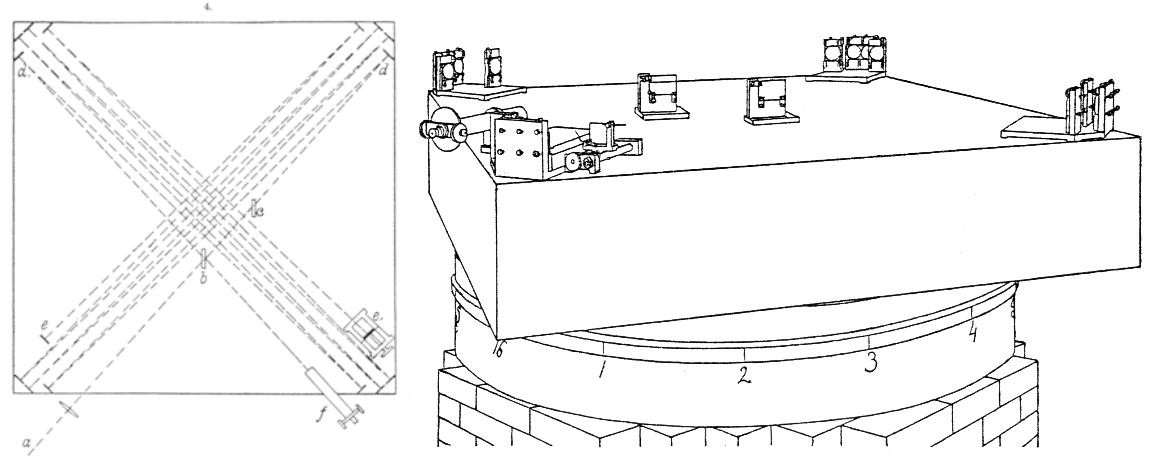
\includegraphics[scale=0.5]{./presentation/cropped-Michelson-morley-header}
%https://araz.community.uaf.edu/

Fig. 2: Principe et dispositif de l'expérience historique de Michelson-Morley.

{\it a : source lumineuse, b : lame semi-transparente, c : lame compensatrice, d : miroirs fixes, e : miroir réglable, f : occulaire}
\end{center}
\begin{enumerate}
  \item Effectuer un calcul de physique Galiléenne pour déterminer le temps d'aller retour d'un
flash lumineux le long de chacun des deux bras. On supposera que le mouvement de la
Terre coïncide avec la direction de l'un des bras.
  \item En déduire, dans la limite v ≪ c , le déphasage qui devrait être observé en sortie de l'interféromètre lorsqu'on éclaire l'interféromètre en lumière monochromatique. Comment observer
expérimentalement ce déphasage ?
  \item Le résultat de l'expérience historique a donné une absence de déphasage à mieux qu'un
centième de frange. Si l'éther existait, quelle serait sa vitesse maximale par rapport à la
Terre ? Commenter.
\end{enumerate}
\subsection{Désintégration de muons cosmiques}
Les muons sont des particules hargées ayant des propriétés très semblables aux éle trons excepté qu'ils sont plus massifs et instables. On les trouve en abondance dans les rayons cosmiques.
Leur durée de vie moyenne au repos a été mesurée et vaut : $\tau$ 0 = 2, 197 × 10 −6 s .
Un détecteur de muons est placé tout d'abord au sommet du Mont Washington (1910 m), puis
au pied de ette montagne, sensiblement au niveau de la mer. Dans sa première position, le
détecteur enregistre 563 +
− 10 muons par heure, dans sa seconde position, 408 +
− 9 .
\begin{enumerate}
  \item En faisant l'hypothèse que la vitesse des muons est proche de c , calculez leur durée de vie
moyenne $\tau$ telle qu'elle est mesurée par un expérimentateur terrestre.
En réalité, au cours de cette expérience, on a pu sélectionner des muons de vitesse v = 0, 992c .
  \item Montrez que l'expérimentateur peut retrouver cette valeur de $\tau$ à partir de la connaissance
de $\tau$ 0 .
\end{enumerate}
\subsection{Temps propre et temps impropre}
Une fusée quitte la Terre avec une vitesse $\beta$ ≡ v/c = 3/5 . Quand une horloge placée sur la
fusée indique qu'une heure s'est écoulée, la fusée envoie un signal lumineux à la Terre.
\begin{enumerate}
  \item Pour les horloges terrestres, quand le signal lumineux a-t-il été envoyé ?
  \item Pour les horloges terrestres, combien de temps après le départ de la fusée le signal a-t-il
atteint la Terre ?
  \item Pour les horloges de la fusée, combien de temps après le départ de la fusée le signal a-t-il
atteint la Terre ?
\end{enumerate}
\subsection{L'effet Doppler}
On considère une source ponctuelle S émettant des flashs lumineux sphériques à une fréquence
qui se propagent à la vitesse de la lumière c . Comme il est indiqué sur la Fig. 3, la source est
animée d'une vitesse v par rapport au référentiel du laboratoire, qui fait un angle $\theta$ avec l'axe
de visée (toujours dans le référentiel du laboratoire).
$\nu$ S '
S
v
q
r
O
Fig. 3 : Source S se déplaçant à la vitesse v par rapport à un observateur O fixe dans le référentiel
du laboratoire.
Un observateur immobile dans ce référentiel est placé au point O. On repère par le vecteur
r la position de la source qui a émis le signal présent en O. On suppose l'observateur éloigné,
c'est-à-dire r ≫ c/$\nu$ ' .
\subsubsection{Effet Doppler classique ( v ≪ c )}
\begin{enumerate}
  \item Dans le référentiel du laboratoire, exprimer la durée ∆t O séparant la réception de 2 flashs
pour l'observateur en fonction de ∆t S , période d'émission du signal dans le référentiel de
l'observateur.
  \item Interpréter graphiquement l'effet Doppler classique en représentant les crêtes correspondant
à 4 périodes successives sur un dessin. Y-a-t-il un effet Doppler classique transverse (pour
$\theta$ = $\pi$/2 ) ?
\setcounter{numero}{\theenumi}\end{enumerate}
\subsubsection{Effet Doppler relativiste}
\begin{enumerate}
  \setcounter{enumi}{\thenumero}
  \item Définir ensuite un référentiel dans lequel l'intervalle de temps séparant 2 flashs est un temps
propre et en déduire la fréquence $\nu$ O mesurée par l'observateur en fonction de v , $\theta$ et de la
fréquence $\nu$ S ' de la source.
\end{enumerate} 
\subsection{Diverses mesures de longueurs}
On considère une fusée voyageant à la vitesse v entre 2 planètes A et B séparées d'une distance L .
\begin{enumerate}
  \item Calculez l'intervalle de temps mesuré par une horloge de la fusée entre les 2 franchissements
de planètes.
  \item Déduisez en la longueur L ' mesurée par le pilote de la fusée entre les 2 planètes.
\setcounter{numero}{\theenumi}\end{enumerate}
On considère un appareil comportant une source d'éclairs E placée à égale distance de 2 miroirs
situés en A et B , eux-mêmes séparés d'une distance L (mesurée au repos). Comme il est indiqué
sur la figure 4, l'ensemble se déplace à une vitesse v par rapport au laboratoire.

La source émet un éclair au temps t = t ' = 0 juste quand elle passe devant le point E ' du
laboratoire. L'éclair atteint les points A et B , est réfléchi vers le laboratoire et laisse 2 marques
en A ' et B ' .
\begin{enumerate}
  \setcounter{enumi}{\thenumero}
  \item Trouvez les temps indiqués par des horloges situées en A , B , A ' et B ' quand l'éclair y arrive.
  \item Les événements : l'éclair est en A ' et l'éclair est en B ' sont-ils simultanés ?
\end{enumerate} 
Fig. 4 : Dispositif émettant un éclair en E et le réfléchissant en A et B .

%\input{/corriges/td0.tex}

%
%====================== INCLUSION DE LA BIBLIOGRAPHIE ======================
%
%récupérer les citation avec "/footnotemark" : 
\nocite{*}
%
% choix du style de la biblio
\bibliographystyle{plain}
%
% inclusion de la biblio
\cleardoublepage
\addcontentsline{toc}{chapter}{Bibliographie}
\bibliography{bibliographie.bib}
%
%====================== FIN DU DOCUMENT ======================
%
\end{document}
%%%%%%%%%%%%%%%%%%%%%%%%%%%%%%%%%%%%%%%%%%%%%%%%%%%%%%%%%%%%%%%%%%%%%%%%%%%%%%%%%
